% Innehåll: resultat och analys.
% I vissa fall kan man ha ”Resultat och diskussion” som kapitel.

%Detta är förmodligen den största delen av rapporten. Här redovisas resultaten rakt på sak på ett objektivt/neutralt sätt. Ofta är det lämpligt att dela upp texten i ett antal underrubriker. Materialet måste presenteras i logisk ordning, vilket inte behöver vara den ordning i vilken försöket/arbetet har utförts.

%Läsaren skall kunna läsa rapporten utan att behöva bläddra fram och tillbaka. Det ska vara tydligt vad som är data respektive analys av data.
%Visas resultat i tabell- eller figurform så måste kortfattat beskrivas vad man ser i figurerna/tabellerna. De placeras i närheten (efter) där de först refererades.

%Som exempel visas fyra mätningar där variabel, 1, varierades. Resultat visas i tabell \ref{tvariabel123} nedan.

% Det skall alltid finnas en tabelltext som förklarar vad som finns i tabellen. Tabellnummer och text ska stå ovanför tabellen.
\subsection{Spike based algorithms}
The algorithm was tested on 8 recordings from three patients, whit a derivative threshold tuned by analysis of the interictal period. The resulting predictions and their accuracy can be seen in the tables(\ref{Der1}-\ref{Der3})

%for the first patient, the algorithm got a precision of $0.33$, a miss rate of $0$, and sensitivity of $1$.The second patient had 


\begin{table}[H]
\centering
    \begin{tabular}{c | c |c |c | c}
        \hline
         file &  FP (timestamps) & TP (timestamps) & NP (timestamps) & (seizure time)  \\
        \hline
        chb1-01 & (180) & Null & Null & Null   \\
        chb1-02 & (180,1620) & Null & Null & Null \\
        chb1-03 & Null & (2160,2520,2700) & Null & (2996)
        \\
        chb1-04	&  Null &   (1260) & Null & (1467)\\
        chb1-05 &   (360,1620) & Null & Null & Null\\
        chb1-06 &   (1440) & Null & Null & Null\\
        chb1-07 &   (1260,900) & Null & Null & Null  \\
        chb1-08 &   (1260) & Null & Null & Null  \\
        \hline
     \end{tabular} 
\caption{Patient number 1, whit criteria set as $2< der < \infty$ }
\label{Der1}
\end{table}

\begin{table}[H]
\centering
    \begin{tabular}{c | c |c |c | c}
        \hline
         file &  FP (timestamps) & TP (timestamps) & NP (timestamps) & (seizure time)  \\
        \hline
        chb2-01 & Null & Null & Null  & Null  \\
        chb2-02 & Null & Null & Null & Null \\
        chb2-03 & Null & Null & Null & Null  \\
        chb2-04	& Null & Null & Null & Null\\
        chb2-05 & Null & Null & Null & Null\\
        chb2-06 & (180,360,1620) & Null & Null & Null\\
        chb2-07 &  Null & Null & Null & Null  \\
        chb2-08 &  Null & Null & Null & Null  \\
        \hline
     \end{tabular} 
\caption{Patient number 2, whit a criteria set as $2< der < \infty$ }
\label{Der2}
\end{table}


\begin{table}[H]
\centering
    \begin{tabular}{c | c |c |c | c}
        \hline
         file &  FP (timestamps) & TP (timestamps) & FN (timestamps) & (seizure time)  \\
        \hline
        chb3-01 & (375) & Null & (362)  & (362)  \\
        chb3-02 & (1080) & (360,720) & Null & (731) \\
        chb3-03 & (1080,1260,1440,1980)& Null & (432) & (432)  \\
       chb3-04	& Null & (180), & Null & (2162)\\
        chb3-05 & Null & Null & Null & Null\\
        chb3-06 & Null & Null & Null & Null\\
        chb3-07 &  Null & Null & Null & Null  \\
        chb3-08 &  Null & Null & Null & Null  \\
        \hline
     \end{tabular} 
\caption{Patient number 3, whit a criteria set as $-0.03< der < 0.05$ }
\label{Der3}
\end{table}


The spike frequency method was tuned by measuring the maximum interictal period across all channels in the first seizure free file of the respective patient. The result is shown in the tables(\ref{Freq1}-\ref{Freq6}).Note that some of the false positives is not a true miss,it hits the seizure, it is merely that it failed to predict it. The maximum spike frequency of the inter-ictal period was aproximately $1.2857$ for patient 1, $3.5714$ for patient 2 and $0.85714$ for patient 3.

\begin{table}[H]
\centering
    \begin{tabular}{c | c |c |c | c}
        \hline
         file &  FP (timestamps) & TP (timestamps) & NP (timestamps) & (seizure time)  \\
        \hline
        chb1-01 & Null & Null & Null  & Null  \\
        chb1-02 & Null & Null & Null & Null \\
        chb1-03 & (3020) & (2995) & Null & (2996) \\
        chb1-04	& (1470) & Null & (1467) & (1467)\\
        chb1-05 & Null & Null & Null & Null\\
        chb1-06 & Null & Null & Null & Null\\
        chb1-07 &  Null & Null & Null & Null  \\
        chb1-08 &  Null & Null & Null & Null  \\
        \hline
     \end{tabular} 
\caption{Patient number 1, with a criteria set as $Spike frequency > 1.2857*1.3$ }
\label{Freq1}
\end{table}
%2.714

\begin{table}[H]
\centering
    \begin{tabular}{c | c |c |c | c}
        \hline
         file &  FP (timestamps) & TP (timestamps) & NP (timestamps) & (seizure time)  \\
        \hline
        chb1-01 & Null & Null & Null  & Null  \\
        chb1-02 & Null & Null & Null & Null \\
        chb1-03 & (805) & (1135) & Null & (2996) \\
        chb1-04	& Null & (1460,1465) & Null & (1467)\\
        chb1-05 & Null & Null & Null & Null\\
        chb1-06 & Null & Null & Null & Null\\
        chb1-07 &  Null & Null & Null & Null  \\
        chb1-08 &  Null & Null & Null & Null  \\
        \hline
     \end{tabular} 
\caption{Patient number 1, with a criteria set as $Spike frequency > 1.2857*1.1$ }
\label{Freq2}
\end{table}

\begin{table}[H]
\centering
    \begin{tabular}{c | c |c |c | c}
        \hline
         file &  FP (timestamps) & TP (timestamps) & NP (timestamps) & (seizure time)  \\
        \hline
        chb2-01 & Null & Null & Null & Null  \\
        chb2-02 & Null & Null & Null & Null \\
        chb2-03 & Null & Null & Null & Null  \\
        chb2-04	& Null & Null & Null & Null\\
        chb2-05 & Null & Null & Null & Null\\
        chb2-06 & Null & Null & Null & Null\\
        chb2-07 &  Null & Null & Null & Null  \\
        chb2-08 &  Null & Null & Null & Null  \\
        \hline
     \end{tabular} 
\caption{Patient number 2, with a criteria set as $Spike frequency > 3.5374*1.3$ }
\label{Freq3}
\end{table}

\begin{table}[H]
\centering
    \begin{tabular}{c | c |c |c | c}
        \hline
         file &  FP (timestamps) & TP (timestamps) & NP (timestamps) & (seizure time)  \\
        \hline
        chb2-01 & Null & Null & Null & Null  \\
        chb2-02 & Null & Null & Null & Null \\
        chb2-03 & Null & Null & Null & Null  \\
        chb2-04	& Null & Null & Null & Null\\
        chb2-05 & Null & Null & Null & Null\\
        chb2-06 & Null & Null & Null & Null\\
        chb2-07 &  Null & Null & Null & Null  \\
        chb2-08 &  Null & Null & Null & Null  \\
        \hline
     \end{tabular} 
\caption{Patient number 2, with a criteria set as $Spike frequency > 3.5374*1.1$ }
\label{Freq4}
\end{table}

\begin{table}[H]
\centering
    \begin{tabular}{c | c |c |c | c}
        \hline
         file &  FP (timestamps) & TP (timestamps) & NP (timestamps) & (seizure time)  \\
        \hline
        chb3-01 & (375,395) & Null & (365) & (365)  \\
        chb3-02 & (755,760) & Null & (731) & (731) \\
        chb3-03 & (445,450,460) & (85,430) & Null & (432)  \\
        chb3-04	& (2170) & Null & (2162) & (2162)\\
        chb3-05 & Null & Null & Null & Null\\
        chb3-06 & Null & Null & Null & Null\\
        chb3-07 &  Null & Null & Null & Null  \\
        chb3-08 &  Null & Null & Null & Null  \\
        \hline
     \end{tabular} 
\caption{Patient number 3, with a criteria set as $Spike frequency > 0.85714*1.3$ }
\label{Freq5}
\end{table}

\begin{table}[H]
\centering
    \begin{tabular}{c | c |c |c | c}
        \hline
         file &  FP (timestamps) & TP (timestamps) & NP (timestamps) & (seizure time)  \\
        \hline
        chb3-01 & (375) & Null & (365) & (365)  \\
        chb3-02 & (755,760) & Null & (731) & (731) \\
        chb3-03 & (450,445,460) & (85,430) & Null & (432)  \\
        chb3-04	& (2170) & Null & (2162) & (2162)\\
        chb3-05 & Null & Null & Null & Null\\
        chb3-06 & Null & Null & Null & Null\\
        chb3-07 &  Null & Null & Null & Null  \\
        chb3-08 &  Null & Null & Null & Null  \\
        \hline
     \end{tabular} 
\caption{Patient number 3, with a criteria set as $Spike frequency > 0.85714*1.1$ }
\label{Freq6}
\end{table}



%Med hjälp av mätvärdena i tabell 1 skapas en produktansats av typen potensfunktion
% där $C, \alpha, ..., \delta$ är konstanter som ska bestämmas experimentellt.
% Avgiven värmemängd från brödrosten (variabel 3) som funktion av tiden variabel 1 visas i figur \ref{fvariabel3vs1}. Den linjära anpassningen i figuren visar att

% och tillförd värmeeffekt till brödrosten bestäms då till 351,8 W.

% Diagram ska ha storhet och enhet på axlarna (SI). Är det tex logaritmerade diagram
% ska de ha storhet (men inte enhet) på axlarna. Figurnummer och text ska stå under
% figur och hänga ihop på samma sida.




\subsection{CNN}



%Neural network (notes)

%70-80\% accuracy on test set

%still not working properly on a continuous stream of data

%works somewhat ok on the continuous data on timeframes from which training data was drawn.

%does not work across multiple occasions or across multiple people, which means that the model isn't general enough, but it still adapts to the existing dataset

%why is that?

%likely because the model is adapting to the noise difference of the different occasions, and that is apparently more prevalent than the difference in states.

%Vad är då vårt resultat?

%Jo, med väldigt hög pricksäkerhet, ofta över 75\%, lyckas nätverket gissa på aldrig tidigare sedd data från test-settet. Det är ju helt fantastiskt, och allt som återstår nu är att testa nätverket i ett “riktigt” scenario, där vi kontinuerligt kör nätverket över en hel session och försöker förutspå ett stundande anfall. Funkar det?

%Nja, kanske. Här syns inget tydligt sammanhang förutom 5 minuter innan anfallet, och detta är “nedsmutsade” resultat, då denna instans av nätverket har fått träna på data från dessa 5 minuter.

%Intressantare vore att göra om datasettet men exkludera dessa 2 anfall.

%Och det kan vi se här. Detta är legitima resultat, men problemet är att det inte längre går att se någon tydlig indikation på att ett anfall är på väg att hända, i alla fall inte inom de tidsramar som vi satt. Men, som vi har plottat det nu så är det vikten för pre-iktalt stadie minus vikten för inter-iktalt stadie. Plotten ger alltså positivt när nätverket tror att en anfall ska ske, och negativt när det inte tror det. Här kommer bilder på sessioner där inget anfall skett.

%Intressant nog så är gissningen nära noll på ena, och kraftigt negativ på andra. Är detta en indikation på att nätverket fungerar? Det är svårt att säga. Hur som helst fungerar det inte som vi förväntar oss att det ska fungera, åtminstone inte inom samma tidsram.

%Slutligen kan vi konstatera att just detta nätverk inte fungerar på nästa patient. Här ser vi individualiteten in action, gissningen verkar helt omvänd.

The CNN is trained on a dataset that contains over 20 hours of data from patient chb1 from the CHB-MIT dataset, compressed into 43200 labelled datawindows. The network was trained and retrained many times with slight modifications. \\

The network has a high accuracy on the test set, about often above 75\%. This means that the network successfully adapts to the dataset, and can predict the epileptic states of the never before seen test set with high accuracy. \\

To further investigate, a simulated scenario meant to represent real life was set up. This works by taking the prediction for pre-ictal, and subtracting the prediction for inter-ictal, and then averaging over time. This yields a graph that can be investigated to visually determine the performance of the network. \\

At first, the simulated scenarios were done on data from the same EEG sessions that the network trained on. The results of that can be seen in figure (\ref{pre_both}).

\begin{figure}[H]
\centering
\begin{subfigure}{0.5\textwidth}
  \centering
  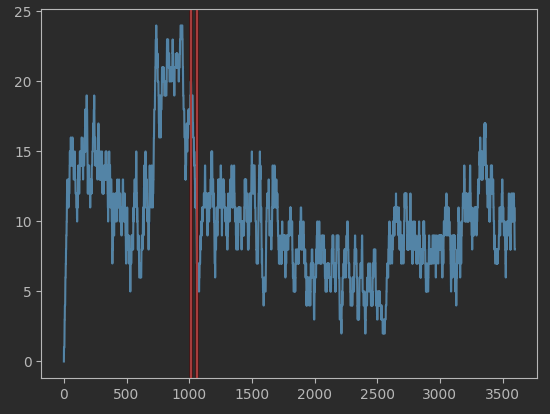
\includegraphics[width=0.9\textwidth]{images/f1-1.png}
  \caption{}
  \label{pre_sub1}
\end{subfigure}%
\begin{subfigure}{0.5\textwidth}
  \centering
  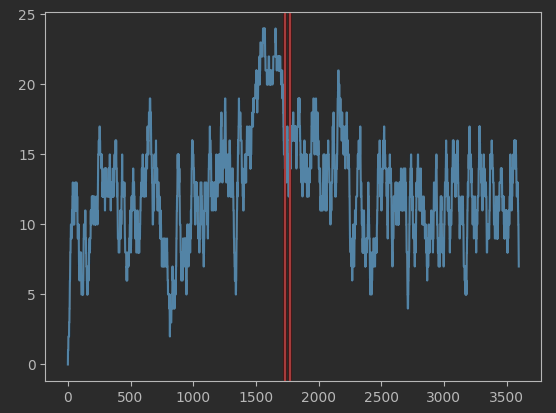
\includegraphics[width=0.9\textwidth]{images/f1-2.png}
  \caption{}
  \label{pre_sub2}
\end{subfigure}
\caption{The results of running a trained network through a simulated scenario meant to represent real life, using data that has been trained on.}
\label{pre_both}
\end{figure}

The result from figure (\ref{pre_both}) clearly increases before the seizure, but it is not presentable as a ``real" result, since it uses data from the same occasions both in the training and to validate itself. To get a proper test, the network has to be retrained on a new dataset, omitting the occasions that will later be used for the visual validation. The results of that can be seen in figure (\ref{real_both}).

\begin{figure}[H]
\centering
\begin{subfigure}{0.5\textwidth}
  \centering
  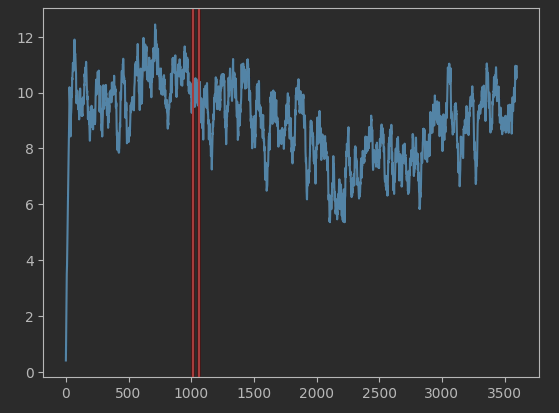
\includegraphics[width=0.9\textwidth]{images/f2-1.png}
  \caption{}
  \label{real_sub1}
\end{subfigure}%
\begin{subfigure}{0.5\textwidth}
  \centering
  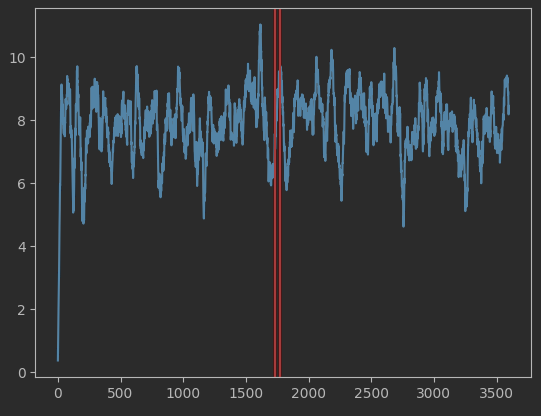
\includegraphics[width=0.9\textwidth]{images/f2-2.png}
  \caption{}
  \label{real_sub2}
\end{subfigure}
\begin{subfigure}{0.5\textwidth}
  \centering
  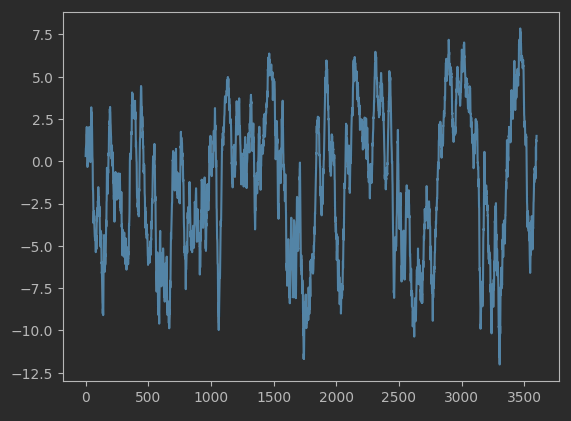
\includegraphics[width=0.9\textwidth]{images/f2-3.png}
  \caption{}
  \label{real_no_sub1}
\end{subfigure}%
\begin{subfigure}{0.5\textwidth}
  \centering
  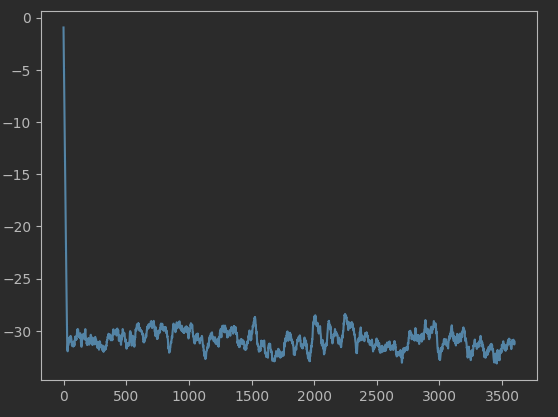
\includegraphics[width=0.9\textwidth]{images/f2-4.png}
  \caption{}
  \label{real_no_sub2}
\end{subfigure}
\caption{The results of running a trained network through a simulated scenario meant to represent real life, without using data that has been trained on.}
\label{real_both}
\end{figure}

As can be seen in figure (\ref{real_both}), when putting the network into this ``real" scenario, the network stops performing well. Instead of seeing an increasing amount of predictions for pre-ictal states closer to the seizure, the prediction distribution seems to be relatively stable throughout the test. However, a pattern still emerges. In data collection occasions where a seizure did occur, the average prediction sum seems much higher than in the occasions where no seizures occurred. \\

For a final test, the network was tested on another patient, chb03 from the CHB-MIT dataset. The results can be seen in figure (\ref{other_both}).

\begin{figure}[H]
\centering
\begin{subfigure}{0.5\textwidth}
  \centering
  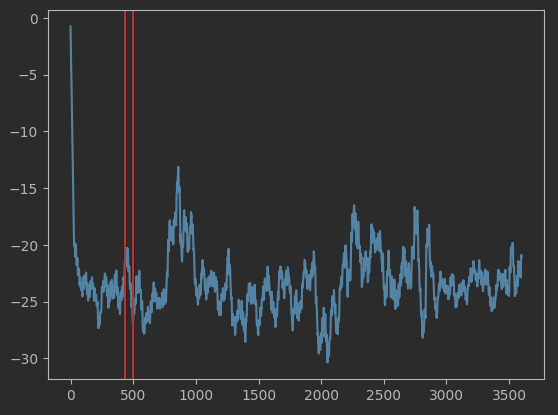
\includegraphics[width=0.9\textwidth]{images/f3-1.png}
  \caption{}
  \label{other_sub1}
\end{subfigure}%
\begin{subfigure}{0.5\textwidth}
  \centering
  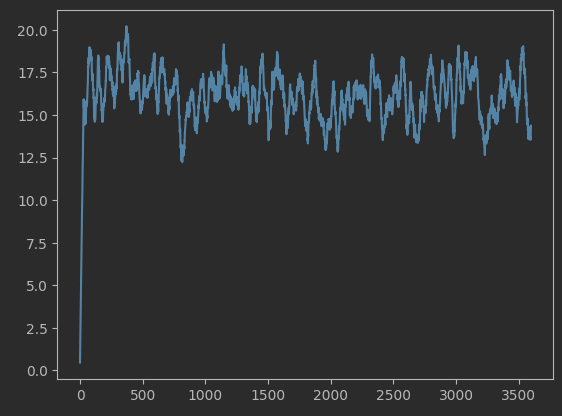
\includegraphics[width=0.9\textwidth]{images/f3-2.png}
  \caption{}
  \label{other_sub2}
\end{subfigure}
\caption{The results of running a trained network through a simulated scenario meant to represent real life, run on another patient than the one trained on.}
\label{other_both}
\end{figure}

The results from figure (\ref{other_both}) are the exact opposite of what was expected. The network predicts inter-ictal throughout a test occasion where a seizure is happening and pre-ictal throughout a test occasion where no seizure occurs. This is a clear indication that the network does not work on a patient it has not trained on.

\subsection{Hardware}
The data processing board from the figure (\ref{fig:PCBData}) in Appendix(\ref{circpart}) is tested in a simulation environment and performs as expected. It is tested with the spike detection algorithm and gets the same result as if it were run on a computer. The UART communication works, but it seems to be some error with the digital isolator, which we have not been able to solve. Assessment of the rest of the circuitry from Appendix(\ref{circpart}) is done both in simulation when possible and primarily by building the circuits on a breadboard and testing them individually. Figure (\ref{fig:ampsim}) shows a simulation plot of the amplification. An input of \SI{10}{\micro\volt} is used, and it produces an output with a max amplitude of \SI{130}{\milli\volt}, which should be sufficient for the ADCs. The amplifier is also tested using a PI-attenuator and a signal generator to test the circuitry with signals in the desired range. From the test, it can be concluded that the amplifier works as intended, but tuning the gain by varying $R_G$ or adding more gain to the buffer stage could be needed, but it needs to be tuned in on the final circuit. All the filters are tested in the same manner and perform as expected. Sadly, the state of the current semiconductor market and delays made it impossible to finish the final circuit at the time of the project course, so no final test with the electrode was run. But since all stages except for the ADCs, which did not arrive in time, are tested separately and work, it is reasonable to assume that the current designs should work but would perhaps need some tuning to get optimal readings.
\begin{figure} [H]
\begin{center}
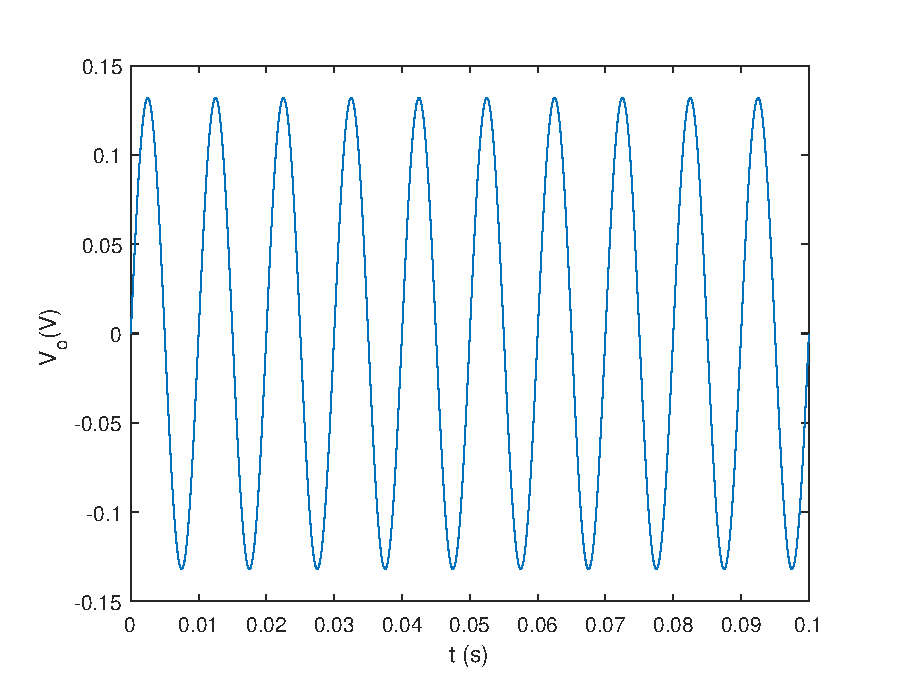
\includegraphics[scale=0.8]{images/Ampout.eps}
   \caption{Simulation of instrumentation amplifier with a input of \SI{10}{\micro\volt}}
    \label{fig:ampsim}
\end{center}
\end{figure}


